\documentclass[twoside]{book}

% Packages required by doxygen
\usepackage{calc}
\usepackage{doxygen}
\usepackage{graphicx}
\usepackage[utf8]{inputenc}
\usepackage{makeidx}
\usepackage{multicol}
\usepackage{multirow}
\usepackage{textcomp}
\usepackage[table]{xcolor}

% Font selection
\usepackage[T1]{fontenc}
\usepackage{mathptmx}
\usepackage[scaled=.90]{helvet}
\usepackage{courier}
\usepackage{amssymb}
\usepackage{sectsty}
\renewcommand{\familydefault}{\sfdefault}
\allsectionsfont{%
  \fontseries{bc}\selectfont%
  \color{darkgray}%
}
\renewcommand{\DoxyLabelFont}{%
  \fontseries{bc}\selectfont%
  \color{darkgray}%
}

% Page & text layout
\usepackage{geometry}
\geometry{%
  a4paper,%
  top=2.5cm,%
  bottom=2.5cm,%
  left=2.5cm,%
  right=2.5cm%
}
\tolerance=750
\hfuzz=15pt
\hbadness=750
\setlength{\emergencystretch}{15pt}
\setlength{\parindent}{0cm}
\setlength{\parskip}{0.2cm}
\makeatletter
\renewcommand{\paragraph}{%
  \@startsection{paragraph}{4}{0ex}{-1.0ex}{1.0ex}{%
    \normalfont\normalsize\bfseries\SS@parafont%
  }%
}
\renewcommand{\subparagraph}{%
  \@startsection{subparagraph}{5}{0ex}{-1.0ex}{1.0ex}{%
    \normalfont\normalsize\bfseries\SS@subparafont%
  }%
}
\makeatother

% Headers & footers
\usepackage{fancyhdr}
\pagestyle{fancyplain}
\fancyhead[LE]{\fancyplain{}{\bfseries\thepage}}
\fancyhead[CE]{\fancyplain{}{}}
\fancyhead[RE]{\fancyplain{}{\bfseries\leftmark}}
\fancyhead[LO]{\fancyplain{}{\bfseries\rightmark}}
\fancyhead[CO]{\fancyplain{}{}}
\fancyhead[RO]{\fancyplain{}{\bfseries\thepage}}
\fancyfoot[LE]{\fancyplain{}{}}
\fancyfoot[CE]{\fancyplain{}{}}
\fancyfoot[RE]{\fancyplain{}{\bfseries\scriptsize Generated on Thu Mar 6 2014 18\-:46\-:55 for Concurrent\-D\-X by Doxygen }}
\fancyfoot[LO]{\fancyplain{}{\bfseries\scriptsize Generated on Thu Mar 6 2014 18\-:46\-:55 for Concurrent\-D\-X by Doxygen }}
\fancyfoot[CO]{\fancyplain{}{}}
\fancyfoot[RO]{\fancyplain{}{}}
\renewcommand{\footrulewidth}{0.4pt}
\renewcommand{\chaptermark}[1]{%
  \markboth{#1}{}%
}
\renewcommand{\sectionmark}[1]{%
  \markright{\thesection\ #1}%
}

% Indices & bibliography
\usepackage{natbib}
\usepackage[titles]{tocloft}
\setcounter{tocdepth}{3}
\setcounter{secnumdepth}{5}
\makeindex

% Hyperlinks (required, but should be loaded last)
\usepackage{ifpdf}
\ifpdf
  \usepackage[pdftex,pagebackref=true]{hyperref}
\else
  \usepackage[ps2pdf,pagebackref=true]{hyperref}
\fi
\hypersetup{%
  colorlinks=true,%
  linkcolor=blue,%
  citecolor=blue,%
  unicode%
}

% Custom commands
\newcommand{\clearemptydoublepage}{%
  \newpage{\pagestyle{empty}\cleardoublepage}%
}


%===== C O N T E N T S =====

\begin{document}

% Titlepage & ToC
\hypersetup{pageanchor=false}
\pagenumbering{roman}
\begin{titlepage}
\vspace*{7cm}
\begin{center}%
{\Large Concurrent\-D\-X \\[1ex]\large 0.\-1 }\\
\vspace*{1cm}
{\large Generated by Doxygen 1.8.6}\\
\vspace*{0.5cm}
{\small Thu Mar 6 2014 18:46:55}\\
\end{center}
\end{titlepage}
\clearemptydoublepage
\tableofcontents
\clearemptydoublepage
\pagenumbering{arabic}
\hypersetup{pageanchor=true}

%--- Begin generated contents ---
\chapter{Concurrent\-D\-X}
\label{md__r_e_a_d_m_e}
\hypertarget{md__r_e_a_d_m_e}{}
Lightweight (no-\/longer-\/header-\/only) C++ concurrency library

{\itshape Disclaimer\-: I have no idea what I'm doing.}

\section*{Using Concurrent\-D\-X}

Concurrent\-D\-X is a header-\/only library. It relies on some C++ 11 features, however. You will need\-:


\begin{DoxyItemize}
\item A (mostly) C++11 standard-\/compliant C++ compiler (M\-S\-V\-C10 and later works)
\item A copy of this repo
\item To do the following with your project (where the include paths have been set up to point to whatever directory holds the repo)\-:
\end{DoxyItemize}

```c++ \#include $<$Concurrent\-D\-X/\-Concurrent\-D\-X.\-h$>$ ```
\begin{DoxyItemize}
\item ...and that's it! All of the classes and containers are in the D\-X\{\} namespace
\end{DoxyItemize}

\section*{Documentation}

Documentation can be found \href{/html/index.html}{\tt here}. The best way to view the documentation is to clone the repo and open up the html off the disk. 
\chapter{Hierarchical Index}
\section{Class Hierarchy}
This inheritance list is sorted roughly, but not completely, alphabetically\-:\begin{DoxyCompactList}
\item \contentsline{section}{D\-X\-:\-:Barrier}{\pageref{class_d_x_1_1_barrier}}{}
\begin{DoxyCompactList}
\item \contentsline{section}{D\-X\-:\-:Cyclic\-Spin\-Barrier}{\pageref{class_d_x_1_1_cyclic_spin_barrier}}{}
\item \contentsline{section}{D\-X\-:\-:Spin\-Barrier}{\pageref{class_d_x_1_1_spin_barrier}}{}
\end{DoxyCompactList}
\item \contentsline{section}{D\-X\-:\-:Mutex}{\pageref{class_d_x_1_1_mutex}}{}
\begin{DoxyCompactList}
\item \contentsline{section}{D\-X\-:\-:Spin\-Mutex}{\pageref{class_d_x_1_1_spin_mutex}}{}
\begin{DoxyCompactList}
\item \contentsline{section}{D\-X\-:\-:Spin\-Recursive\-Mutex}{\pageref{class_d_x_1_1_spin_recursive_mutex}}{}
\item \contentsline{section}{D\-X\-:\-:Spin\-Yield\-Mutex}{\pageref{class_d_x_1_1_spin_yield_mutex}}{}
\end{DoxyCompactList}
\end{DoxyCompactList}
\item \contentsline{section}{D\-X\-:\-:Node$<$ T $>$}{\pageref{struct_d_x_1_1_node}}{}
\item \contentsline{section}{D\-X\-:\-:Queue$<$ T $>$}{\pageref{class_d_x_1_1_queue}}{}
\begin{DoxyCompactList}
\item \contentsline{section}{D\-X\-:\-:Concurrent\-Queue$<$ T $>$}{\pageref{class_d_x_1_1_concurrent_queue}}{}
\item \contentsline{section}{D\-X\-:\-:Concurrent\-Stream$<$ T $>$}{\pageref{class_d_x_1_1_concurrent_stream}}{}
\end{DoxyCompactList}
\item \contentsline{section}{D\-X\-:\-:Spin\-Lock}{\pageref{class_d_x_1_1_spin_lock}}{}
\item \contentsline{section}{D\-X\-:\-:Spin\-R\-W\-Lock}{\pageref{class_d_x_1_1_spin_r_w_lock}}{}
\item \contentsline{section}{D\-X\-:\-:Spin\-R\-W\-Mutex}{\pageref{class_d_x_1_1_spin_r_w_mutex}}{}
\item \contentsline{section}{D\-X\-:\-:Std\-Lock}{\pageref{class_d_x_1_1_std_lock}}{}
\end{DoxyCompactList}

\chapter{Class Index}
\section{Class List}
Here are the classes, structs, unions and interfaces with brief descriptions\-:\begin{DoxyCompactList}
\item\contentsline{section}{\hyperlink{class_d_x_1_1_barrier}{D\-X\-::\-Barrier} }{\pageref{class_d_x_1_1_barrier}}{}
\item\contentsline{section}{\hyperlink{class_d_x_1_1_concurrent_queue}{D\-X\-::\-Concurrent\-Queue$<$ T $>$} }{\pageref{class_d_x_1_1_concurrent_queue}}{}
\item\contentsline{section}{\hyperlink{class_d_x_1_1_concurrent_stream}{D\-X\-::\-Concurrent\-Stream$<$ T $>$} }{\pageref{class_d_x_1_1_concurrent_stream}}{}
\item\contentsline{section}{\hyperlink{class_d_x_1_1_cyclic_spin_barrier}{D\-X\-::\-Cyclic\-Spin\-Barrier} }{\pageref{class_d_x_1_1_cyclic_spin_barrier}}{}
\item\contentsline{section}{\hyperlink{class_d_x_1_1_lock}{D\-X\-::\-Lock} }{\pageref{class_d_x_1_1_lock}}{}
\item\contentsline{section}{\hyperlink{class_d_x_1_1_mutex}{D\-X\-::\-Mutex} }{\pageref{class_d_x_1_1_mutex}}{}
\item\contentsline{section}{\hyperlink{struct_d_x_1_1_node}{D\-X\-::\-Node$<$ T $>$} }{\pageref{struct_d_x_1_1_node}}{}
\item\contentsline{section}{\hyperlink{class_d_x_1_1_queue}{D\-X\-::\-Queue$<$ T $>$} }{\pageref{class_d_x_1_1_queue}}{}
\item\contentsline{section}{\hyperlink{class_d_x_1_1_spin_barrier}{D\-X\-::\-Spin\-Barrier} }{\pageref{class_d_x_1_1_spin_barrier}}{}
\item\contentsline{section}{\hyperlink{class_d_x_1_1_spin_lock}{D\-X\-::\-Spin\-Lock} \\*\hyperlink{class_d_x_1_1_spin_lock}{Spin\-Lock} is a lock-\/guard style class that latches onto a mutex, locking it upon creation and unlocking it upon destruction }{\pageref{class_d_x_1_1_spin_lock}}{}
\item\contentsline{section}{\hyperlink{class_d_x_1_1_spin_mutex}{D\-X\-::\-Spin\-Mutex} \\*\hyperlink{class_d_x_1_1_spin_mutex}{Spin\-Mutex} is a leightweight mutex class that makes use of C++11 atomics to spin out in active-\/\-C\-P\-U-\/land as opposed to the traditional method of yielding context. It's target use-\/case is for code regions that aren't too highly contended, or for contended regions that execute fairly fast }{\pageref{class_d_x_1_1_spin_mutex}}{}
\item\contentsline{section}{\hyperlink{class_d_x_1_1_spin_recursive_mutex}{D\-X\-::\-Spin\-Recursive\-Mutex} }{\pageref{class_d_x_1_1_spin_recursive_mutex}}{}
\item\contentsline{section}{\hyperlink{class_d_x_1_1_spin_r_w_lock}{D\-X\-::\-Spin\-R\-W\-Lock} \\*\hyperlink{class_d_x_1_1_spin_r_w_lock}{Spin\-R\-W\-Lock} is the preferred way of interacting with a \hyperlink{class_d_x_1_1_spin_r_w_mutex}{Spin\-R\-W\-Mutex}. \hyperlink{class_d_x_1_1_spin_r_w_lock}{Spin\-R\-W\-Lock} is a lock-\/guard style class, locking the \hyperlink{class_d_x_1_1_spin_r_w_mutex}{Spin\-R\-W\-Mutex} upon construction and releasing the lock upon destruction. \hyperlink{class_d_x_1_1_spin_r_w_mutex}{Spin\-R\-W\-Mutex} remembers whether it is a reader or writer lock, and releases the same kind of lock that it was constructed with }{\pageref{class_d_x_1_1_spin_r_w_lock}}{}
\item\contentsline{section}{\hyperlink{class_d_x_1_1_spin_r_w_mutex}{D\-X\-::\-Spin\-R\-W\-Mutex} \\*\hyperlink{class_d_x_1_1_spin_r_w_mutex}{Spin\-R\-W\-Mutex} is a leightweight mutex that supports multiple readers (const-\/only access) and a single writer. Supports readers up to the maximum value of size\-\_\-t for your system }{\pageref{class_d_x_1_1_spin_r_w_mutex}}{}
\item\contentsline{section}{\hyperlink{class_d_x_1_1_spin_yield_mutex}{D\-X\-::\-Spin\-Yield\-Mutex} }{\pageref{class_d_x_1_1_spin_yield_mutex}}{}
\item\contentsline{section}{\hyperlink{class_d_x_1_1_std_lock}{D\-X\-::\-Std\-Lock} }{\pageref{class_d_x_1_1_std_lock}}{}
\end{DoxyCompactList}

\chapter{Class Documentation}
\hypertarget{class_d_x_1_1_barrier}{\section{D\-X\-:\-:Barrier Class Reference}
\label{class_d_x_1_1_barrier}\index{D\-X\-::\-Barrier@{D\-X\-::\-Barrier}}
}
Inheritance diagram for D\-X\-:\-:Barrier\-:\begin{figure}[H]
\begin{center}
\leavevmode
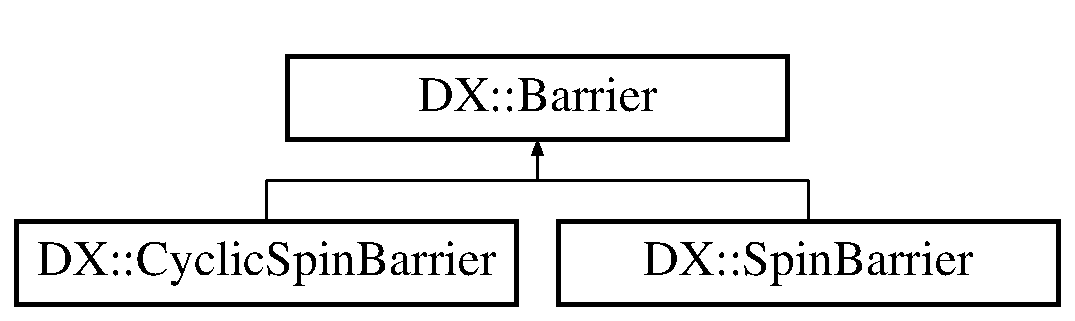
\includegraphics[height=2.000000cm]{class_d_x_1_1_barrier}
\end{center}
\end{figure}
\subsection*{Public Member Functions}
\begin{DoxyCompactItemize}
\item 
\hypertarget{class_d_x_1_1_barrier_ae7a881ba86bd4f16a25600f00457e710}{{\bfseries Barrier} (size\-\_\-t num\-Threads)}\label{class_d_x_1_1_barrier_ae7a881ba86bd4f16a25600f00457e710}

\item 
\hypertarget{class_d_x_1_1_barrier_a34b9c56a632e7ace41532794ff98694d}{virtual void {\bfseries wait} () const =0}\label{class_d_x_1_1_barrier_a34b9c56a632e7ace41532794ff98694d}

\end{DoxyCompactItemize}
\subsection*{Protected Attributes}
\begin{DoxyCompactItemize}
\item 
\hypertarget{class_d_x_1_1_barrier_a39956c1715d3c86fe73861b2fee5065d}{volatile char {\bfseries pad\-\_\-0} \mbox{[}C\-A\-C\-H\-E\-\_\-\-L\-I\-N\-E\-\_\-\-S\-I\-Z\-E\mbox{]}}\label{class_d_x_1_1_barrier_a39956c1715d3c86fe73861b2fee5065d}

\item 
\hypertarget{class_d_x_1_1_barrier_ad9ffd4f0c093bfa7018fd836e4b7d681}{std\-::atomic$<$ size\-\_\-t $>$ {\bfseries m\-\_\-count}}\label{class_d_x_1_1_barrier_ad9ffd4f0c093bfa7018fd836e4b7d681}

\item 
\hypertarget{class_d_x_1_1_barrier_afd62281a71cce98c88af7430bc6442a7}{volatile char {\bfseries pad\-\_\-1} \mbox{[}C\-A\-C\-H\-E\-\_\-\-L\-I\-N\-E\-\_\-\-S\-I\-Z\-E-\/(sizeof(std\-::atomic$<$ size\-\_\-t $>$)\%C\-A\-C\-H\-E\-\_\-\-L\-I\-N\-E\-\_\-\-S\-I\-Z\-E)\mbox{]}}\label{class_d_x_1_1_barrier_afd62281a71cce98c88af7430bc6442a7}

\end{DoxyCompactItemize}


The documentation for this class was generated from the following files\-:\begin{DoxyCompactItemize}
\item 
Mutex/Barrier.\-h\item 
Mutex/Barrier.\-cpp\end{DoxyCompactItemize}

\hypertarget{class_d_x_1_1_concurrent_queue}{\section{D\-X\-:\-:Concurrent\-Queue$<$ T $>$ Class Template Reference}
\label{class_d_x_1_1_concurrent_queue}\index{D\-X\-::\-Concurrent\-Queue$<$ T $>$@{D\-X\-::\-Concurrent\-Queue$<$ T $>$}}
}
\subsection*{Public Member Functions}
\begin{DoxyCompactItemize}
\item 
\hypertarget{class_d_x_1_1_concurrent_queue_a53b572618eefcd822c5f480df1ff0a68}{{\bfseries Concurrent\-Queue} (const \hyperlink{class_d_x_1_1_concurrent_queue}{Concurrent\-Queue} \&copy)}\label{class_d_x_1_1_concurrent_queue_a53b572618eefcd822c5f480df1ff0a68}

\item 
\hypertarget{class_d_x_1_1_concurrent_queue_a97410a1d0d3a36f5ee9715ba39929f01}{{\bfseries Concurrent\-Queue} (\hyperlink{class_d_x_1_1_concurrent_queue}{Concurrent\-Queue} \&\&move)}\label{class_d_x_1_1_concurrent_queue_a97410a1d0d3a36f5ee9715ba39929f01}

\item 
\hypertarget{class_d_x_1_1_concurrent_queue_a471ad014f5c7bbcc7564792be3738e74}{bool {\bfseries is\-Empty} () const }\label{class_d_x_1_1_concurrent_queue_a471ad014f5c7bbcc7564792be3738e74}

\item 
\hypertarget{class_d_x_1_1_concurrent_queue_a8bceba6b265016871335a98ce3985cfb}{size\-\_\-t {\bfseries size} () const }\label{class_d_x_1_1_concurrent_queue_a8bceba6b265016871335a98ce3985cfb}

\item 
\hypertarget{class_d_x_1_1_concurrent_queue_a3506ef7d7ea9b5619818aa8fce507087}{T {\bfseries pop} ()}\label{class_d_x_1_1_concurrent_queue_a3506ef7d7ea9b5619818aa8fce507087}

\item 
\hypertarget{class_d_x_1_1_concurrent_queue_aacd4c07e131e1d562c74fa0d23289ea5}{void {\bfseries push} (const T \&)}\label{class_d_x_1_1_concurrent_queue_aacd4c07e131e1d562c74fa0d23289ea5}

\end{DoxyCompactItemize}


The documentation for this class was generated from the following file\-:\begin{DoxyCompactItemize}
\item 
Containers/Concurrent\-Queue.\-h\end{DoxyCompactItemize}

\hypertarget{class_d_x_1_1_concurrent_stream}{\section{D\-X\-:\-:Concurrent\-Stream$<$ T $>$ Class Template Reference}
\label{class_d_x_1_1_concurrent_stream}\index{D\-X\-::\-Concurrent\-Stream$<$ T $>$@{D\-X\-::\-Concurrent\-Stream$<$ T $>$}}
}
Inheritance diagram for D\-X\-:\-:Concurrent\-Stream$<$ T $>$\-:\begin{figure}[H]
\begin{center}
\leavevmode
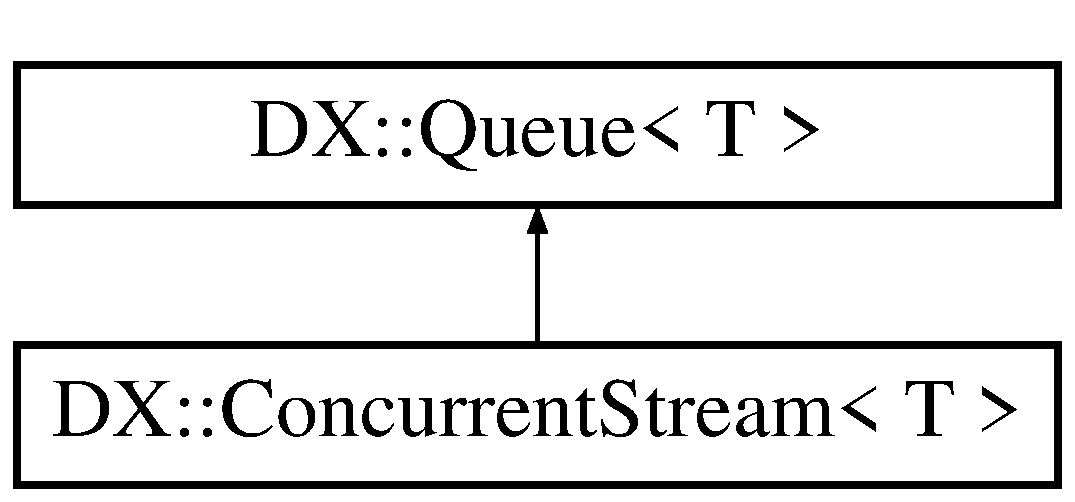
\includegraphics[height=2.000000cm]{class_d_x_1_1_concurrent_stream}
\end{center}
\end{figure}
\subsection*{Public Member Functions}
\begin{DoxyCompactItemize}
\item 
\hypertarget{class_d_x_1_1_concurrent_stream_ac6fcc56db716738fe77ddde565339503}{{\bfseries Concurrent\-Stream} (const \hyperlink{class_d_x_1_1_concurrent_stream}{Concurrent\-Stream} \&)}\label{class_d_x_1_1_concurrent_stream_ac6fcc56db716738fe77ddde565339503}

\item 
\hypertarget{class_d_x_1_1_concurrent_stream_aac12bcb6244dd7e4ae9a62aa785d79c9}{{\bfseries Concurrent\-Stream} (\hyperlink{class_d_x_1_1_concurrent_stream}{Concurrent\-Stream} \&\&)}\label{class_d_x_1_1_concurrent_stream_aac12bcb6244dd7e4ae9a62aa785d79c9}

\item 
\hypertarget{class_d_x_1_1_concurrent_stream_a18a671c877a53863cf37761eadb2a207}{bool {\bfseries is\-Empty} () const }\label{class_d_x_1_1_concurrent_stream_a18a671c877a53863cf37761eadb2a207}

\item 
\hypertarget{class_d_x_1_1_concurrent_stream_a33a0054e52290fdb5df8e6d3a7850768}{size\-\_\-t {\bfseries size} () const }\label{class_d_x_1_1_concurrent_stream_a33a0054e52290fdb5df8e6d3a7850768}

\item 
\hypertarget{class_d_x_1_1_concurrent_stream_a9521bf954d75c36f8ebfb6376a2c203d}{bool {\bfseries pop} (T \&in)}\label{class_d_x_1_1_concurrent_stream_a9521bf954d75c36f8ebfb6376a2c203d}

\item 
\hypertarget{class_d_x_1_1_concurrent_stream_ae25718d47d004e3d213556b9d736d5fe}{void {\bfseries push} (const T \&)}\label{class_d_x_1_1_concurrent_stream_ae25718d47d004e3d213556b9d736d5fe}

\end{DoxyCompactItemize}
\subsection*{Additional Inherited Members}


The documentation for this class was generated from the following file\-:\begin{DoxyCompactItemize}
\item 
Containers/Concurrent\-Stream.\-h\end{DoxyCompactItemize}

\hypertarget{class_d_x_1_1_cyclic_spin_barrier}{\section{D\-X\-:\-:Cyclic\-Spin\-Barrier Class Reference}
\label{class_d_x_1_1_cyclic_spin_barrier}\index{D\-X\-::\-Cyclic\-Spin\-Barrier@{D\-X\-::\-Cyclic\-Spin\-Barrier}}
}
Inheritance diagram for D\-X\-:\-:Cyclic\-Spin\-Barrier\-:\begin{figure}[H]
\begin{center}
\leavevmode
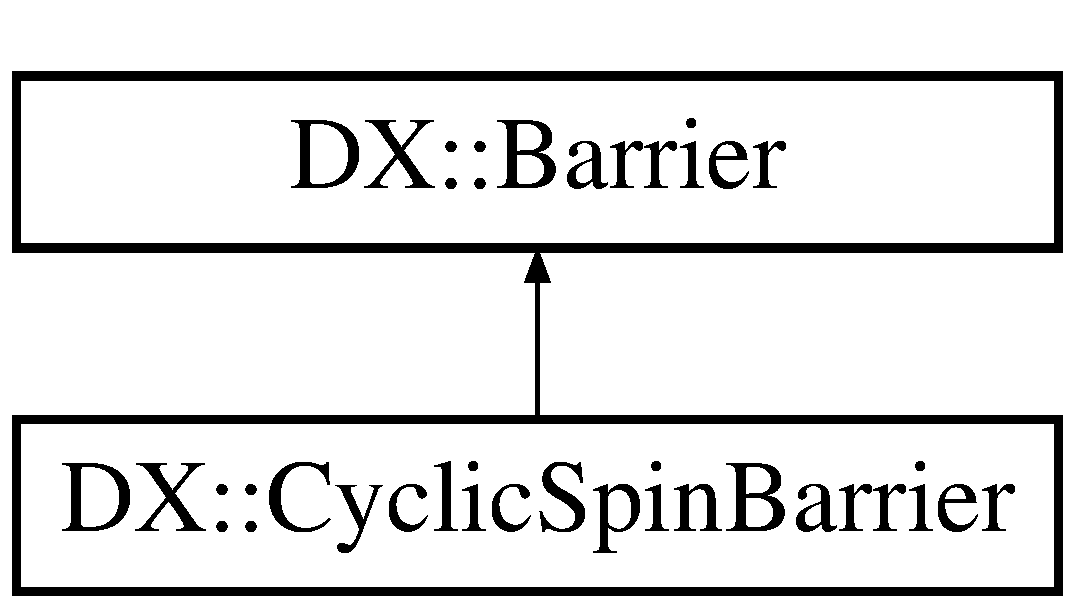
\includegraphics[height=2.000000cm]{class_d_x_1_1_cyclic_spin_barrier}
\end{center}
\end{figure}
\subsection*{Public Member Functions}
\begin{DoxyCompactItemize}
\item 
\hypertarget{class_d_x_1_1_cyclic_spin_barrier_a5450fa600f1c497b4c08d69a0df49929}{{\bfseries Cyclic\-Spin\-Barrier} (size\-\_\-t num\-Threads=1)}\label{class_d_x_1_1_cyclic_spin_barrier_a5450fa600f1c497b4c08d69a0df49929}

\item 
\hypertarget{class_d_x_1_1_cyclic_spin_barrier_abdb6dfc6f2146dce6bcf39718a6f92e5}{void {\bfseries wait} () const }\label{class_d_x_1_1_cyclic_spin_barrier_abdb6dfc6f2146dce6bcf39718a6f92e5}

\end{DoxyCompactItemize}
\subsection*{Additional Inherited Members}


The documentation for this class was generated from the following file\-:\begin{DoxyCompactItemize}
\item 
Mutex/Spin\-Locks.\-h\end{DoxyCompactItemize}

\hypertarget{class_d_x_1_1_mutex}{\section{D\-X\-:\-:Mutex Class Reference}
\label{class_d_x_1_1_mutex}\index{D\-X\-::\-Mutex@{D\-X\-::\-Mutex}}
}
Inheritance diagram for D\-X\-:\-:Mutex\-:\begin{figure}[H]
\begin{center}
\leavevmode
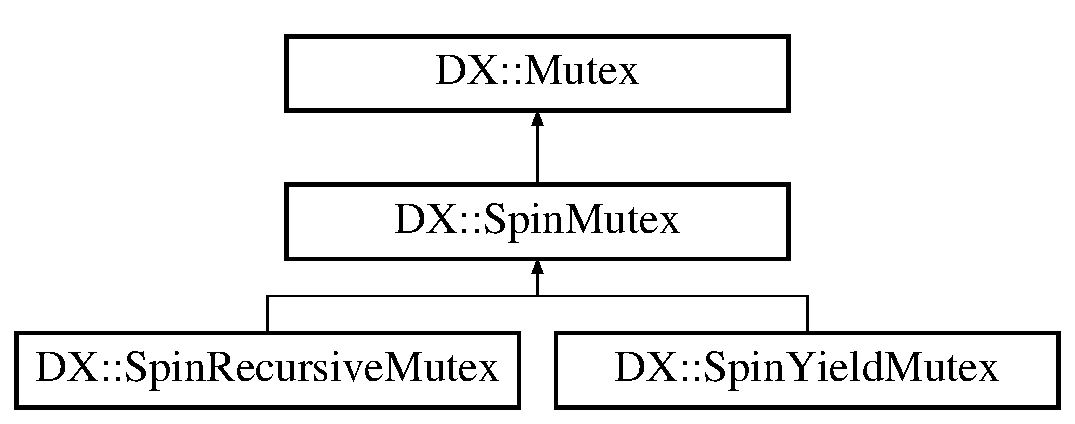
\includegraphics[height=3.000000cm]{class_d_x_1_1_mutex}
\end{center}
\end{figure}
\subsection*{Public Member Functions}
\begin{DoxyCompactItemize}
\item 
\hypertarget{class_d_x_1_1_mutex_aaac9b22f8b25c59db3e22eb1573fc4bf}{virtual void {\bfseries lock} () const =0}\label{class_d_x_1_1_mutex_aaac9b22f8b25c59db3e22eb1573fc4bf}

\item 
\hypertarget{class_d_x_1_1_mutex_a3e89a059beab053e852366a810298073}{virtual void {\bfseries unlock} () const =0}\label{class_d_x_1_1_mutex_a3e89a059beab053e852366a810298073}

\end{DoxyCompactItemize}


The documentation for this class was generated from the following file\-:\begin{DoxyCompactItemize}
\item 
Mutex/Spin\-Locks.\-h\end{DoxyCompactItemize}

\hypertarget{struct_d_x_1_1_node}{\section{D\-X\-:\-:Node$<$ T $>$ Struct Template Reference}
\label{struct_d_x_1_1_node}\index{D\-X\-::\-Node$<$ T $>$@{D\-X\-::\-Node$<$ T $>$}}
}
\subsection*{Public Member Functions}
\begin{DoxyCompactItemize}
\item 
\hypertarget{struct_d_x_1_1_node_a56b09396836fae506175343de2e924ce}{{\bfseries Node} (T $\ast$data)}\label{struct_d_x_1_1_node_a56b09396836fae506175343de2e924ce}

\end{DoxyCompactItemize}
\subsection*{Public Attributes}
\begin{DoxyCompactItemize}
\item 
\hypertarget{struct_d_x_1_1_node_ae52ee669616a0e9dd2f01a687931ca05}{T $\ast$ {\bfseries data}}\label{struct_d_x_1_1_node_ae52ee669616a0e9dd2f01a687931ca05}

\item 
\hypertarget{struct_d_x_1_1_node_a8b9580e73f0f9325898e19bbe36c3dd3}{std\-::atomic$<$ \hyperlink{struct_d_x_1_1_node}{Node} $\ast$ $>$ {\bfseries next}}\label{struct_d_x_1_1_node_a8b9580e73f0f9325898e19bbe36c3dd3}

\item 
\hypertarget{struct_d_x_1_1_node_a6d1d2ba6bff1f20f955c1e8d19212f89}{volatile char {\bfseries pad\-\_\-} \mbox{[}C\-A\-C\-H\-E\-\_\-\-L\-I\-N\-E\-\_\-\-S\-I\-Z\-E-\/((sizeof(T $\ast$)+sizeof(std\-::atomic$<$ \hyperlink{struct_d_x_1_1_node}{Node} $\ast$ $>$))\%C\-A\-C\-H\-E\-\_\-\-L\-I\-N\-E\-\_\-\-S\-I\-Z\-E)\mbox{]}}\label{struct_d_x_1_1_node_a6d1d2ba6bff1f20f955c1e8d19212f89}

\end{DoxyCompactItemize}


The documentation for this struct was generated from the following file\-:\begin{DoxyCompactItemize}
\item 
Containers/Abstract\-Queue.\-h\end{DoxyCompactItemize}

\hypertarget{class_d_x_1_1_queue}{\section{D\-X\-:\-:Queue$<$ T $>$ Class Template Reference}
\label{class_d_x_1_1_queue}\index{D\-X\-::\-Queue$<$ T $>$@{D\-X\-::\-Queue$<$ T $>$}}
}
Inheritance diagram for D\-X\-:\-:Queue$<$ T $>$\-:\begin{figure}[H]
\begin{center}
\leavevmode
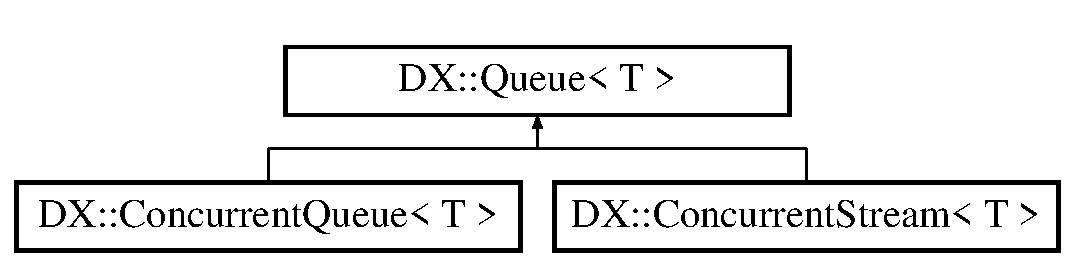
\includegraphics[height=2.000000cm]{class_d_x_1_1_queue}
\end{center}
\end{figure}
\subsection*{Public Member Functions}
\begin{DoxyCompactItemize}
\item 
\hypertarget{class_d_x_1_1_queue_af008aa136485037838cfe0f918792ab9}{virtual bool {\bfseries is\-Empty} () const }\label{class_d_x_1_1_queue_af008aa136485037838cfe0f918792ab9}

\item 
\hypertarget{class_d_x_1_1_queue_adf7128cfd7f99535b4c9a32e22af531e}{virtual size\-\_\-t {\bfseries size} () const }\label{class_d_x_1_1_queue_adf7128cfd7f99535b4c9a32e22af531e}

\item 
\hypertarget{class_d_x_1_1_queue_a37d06d4d1c44ef1393230f0ab995e585}{virtual bool {\bfseries pop} (T \&in)=0}\label{class_d_x_1_1_queue_a37d06d4d1c44ef1393230f0ab995e585}

\item 
\hypertarget{class_d_x_1_1_queue_a1b2b163d92437074055e89837a9414f1}{virtual void {\bfseries push} (const T \&in)=0}\label{class_d_x_1_1_queue_a1b2b163d92437074055e89837a9414f1}

\item 
\hypertarget{class_d_x_1_1_queue_a96ed0255ea3237a9cf66dd7f6aa85a27}{bool {\bfseries operator$>$$>$} (T \&)}\label{class_d_x_1_1_queue_a96ed0255ea3237a9cf66dd7f6aa85a27}

\item 
\hypertarget{class_d_x_1_1_queue_a89202fcd64704521f67b506266d06ec8}{\hyperlink{class_d_x_1_1_queue}{Queue} \& {\bfseries operator$<$$<$} (const T \&)}\label{class_d_x_1_1_queue_a89202fcd64704521f67b506266d06ec8}

\end{DoxyCompactItemize}
\subsection*{Protected Attributes}
\begin{DoxyCompactItemize}
\item 
\hypertarget{class_d_x_1_1_queue_a3e41a2b5013c79a3909f83a2ce65446b}{\hyperlink{struct_d_x_1_1_node}{Node}$<$ T $>$ $\ast$ {\bfseries m\-\_\-start}}\label{class_d_x_1_1_queue_a3e41a2b5013c79a3909f83a2ce65446b}

\item 
\hypertarget{class_d_x_1_1_queue_afb07bbecbb79cce77c0062721a8caa4d}{volatile char {\bfseries pad\-\_\-0} \mbox{[}C\-A\-C\-H\-E\-\_\-\-L\-I\-N\-E\-\_\-\-S\-I\-Z\-E-\/(sizeof(\hyperlink{struct_d_x_1_1_node}{Node}$<$ T $>$ $\ast$)\%C\-A\-C\-H\-E\-\_\-\-L\-I\-N\-E\-\_\-\-S\-I\-Z\-E)\mbox{]}}\label{class_d_x_1_1_queue_afb07bbecbb79cce77c0062721a8caa4d}

\item 
\hypertarget{class_d_x_1_1_queue_a24bd17c6310053ad9e43f84a7d88e5ab}{\hyperlink{struct_d_x_1_1_node}{Node}$<$ T $>$ $\ast$ {\bfseries m\-\_\-end}}\label{class_d_x_1_1_queue_a24bd17c6310053ad9e43f84a7d88e5ab}

\item 
\hypertarget{class_d_x_1_1_queue_a7f9ffb15fb04758bb68af88c676ad4d7}{volatile char {\bfseries pad\-\_\-1} \mbox{[}C\-A\-C\-H\-E\-\_\-\-L\-I\-N\-E\-\_\-\-S\-I\-Z\-E-\/(sizeof(\hyperlink{struct_d_x_1_1_node}{Node}$<$ T $>$ $\ast$)\%C\-A\-C\-H\-E\-\_\-\-L\-I\-N\-E\-\_\-\-S\-I\-Z\-E)\mbox{]}}\label{class_d_x_1_1_queue_a7f9ffb15fb04758bb68af88c676ad4d7}

\item 
\hypertarget{class_d_x_1_1_queue_a4c312cbb0fd52de3cddbf53faec25d49}{std\-::atomic$<$ size\-\_\-t $>$ {\bfseries m\-\_\-size}}\label{class_d_x_1_1_queue_a4c312cbb0fd52de3cddbf53faec25d49}

\item 
\hypertarget{class_d_x_1_1_queue_ae72b76603322862275fa059e1a732d42}{volatile char {\bfseries pad\-\_\-2} \mbox{[}C\-A\-C\-H\-E\-\_\-\-L\-I\-N\-E\-\_\-\-S\-I\-Z\-E-\/(sizeof(std\-::atomic$<$ size\-\_\-t $>$)\%C\-A\-C\-H\-E\-\_\-\-L\-I\-N\-E\-\_\-\-S\-I\-Z\-E)\mbox{]}}\label{class_d_x_1_1_queue_ae72b76603322862275fa059e1a732d42}

\end{DoxyCompactItemize}


The documentation for this class was generated from the following file\-:\begin{DoxyCompactItemize}
\item 
Containers/Abstract\-Queue.\-h\end{DoxyCompactItemize}

\hypertarget{class_d_x_1_1_spin_barrier}{\section{D\-X\-:\-:Spin\-Barrier Class Reference}
\label{class_d_x_1_1_spin_barrier}\index{D\-X\-::\-Spin\-Barrier@{D\-X\-::\-Spin\-Barrier}}
}
Inheritance diagram for D\-X\-:\-:Spin\-Barrier\-:\begin{figure}[H]
\begin{center}
\leavevmode
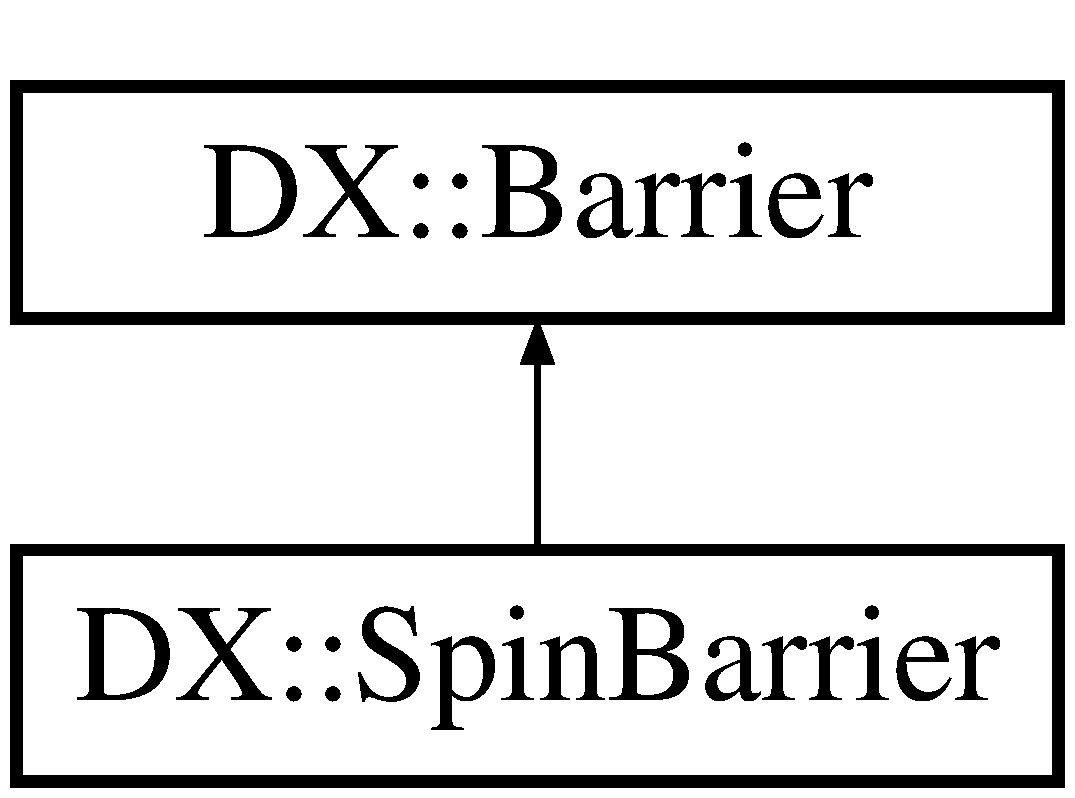
\includegraphics[height=2.000000cm]{class_d_x_1_1_spin_barrier}
\end{center}
\end{figure}
\subsection*{Public Member Functions}
\begin{DoxyCompactItemize}
\item 
\hypertarget{class_d_x_1_1_spin_barrier_a655779e1845cbefa59801553b2eafa2d}{{\bfseries Spin\-Barrier} (size\-\_\-t num\-Threads=1)}\label{class_d_x_1_1_spin_barrier_a655779e1845cbefa59801553b2eafa2d}

\item 
\hypertarget{class_d_x_1_1_spin_barrier_acc73c0fb586ae1694b65d2eb5c50c301}{void {\bfseries wait} () const }\label{class_d_x_1_1_spin_barrier_acc73c0fb586ae1694b65d2eb5c50c301}

\end{DoxyCompactItemize}
\subsection*{Additional Inherited Members}


The documentation for this class was generated from the following files\-:\begin{DoxyCompactItemize}
\item 
Mutex/Spin\-Barrier.\-h\item 
Mutex/Spin\-Barrier.\-cpp\end{DoxyCompactItemize}

\hypertarget{class_d_x_1_1_spin_lock}{\section{D\-X\-:\-:Spin\-Lock Class Reference}
\label{class_d_x_1_1_spin_lock}\index{D\-X\-::\-Spin\-Lock@{D\-X\-::\-Spin\-Lock}}
}


\hyperlink{class_d_x_1_1_spin_lock}{Spin\-Lock} is a lock-\/guard style class that latches onto a mutex, locking it upon creation and unlocking it upon destruction.  




{\ttfamily \#include $<$Spin\-Mutex.\-h$>$}

\subsection*{Public Member Functions}
\begin{DoxyCompactItemize}
\item 
\hyperlink{class_d_x_1_1_spin_lock_a338ff0b08d3517e734fbf190bfff7e24}{Spin\-Lock} (const \hyperlink{class_d_x_1_1_spin_mutex}{Spin\-Mutex} \&mutex)
\end{DoxyCompactItemize}


\subsection{Detailed Description}
\hyperlink{class_d_x_1_1_spin_lock}{Spin\-Lock} is a lock-\/guard style class that latches onto a mutex, locking it upon creation and unlocking it upon destruction. 

Spin\-Locks are the preferred way of interacting with \hyperlink{class_d_x_1_1_spin_mutex}{Spin\-Mutex}.

\begin{DoxyNote}{Note}
Spin\-Locks do not allow for recursive locking of a \hyperlink{class_d_x_1_1_spin_mutex}{Spin\-Mutex}
\end{DoxyNote}
Here are two examples of using Spin\-Locks to protect critical sections of code\-: 
\begin{DoxyCode}
MyClass myClass;
SpinMutex myMutex;

\textcolor{keywordtype}{void} getMyClass()\textcolor{keyword}{ const}
\textcolor{keyword}{}\{
    \hyperlink{class_d_x_1_1_spin_lock_a338ff0b08d3517e734fbf190bfff7e24}{SpinLock} \_lock(myMutex);
    \textcolor{keywordflow}{return} myClass; \textcolor{comment}{// After the return, \_lock destroys itself, automatically unlocking myMutex}
\}
\end{DoxyCode}



\begin{DoxyCode}
MyClass myClass;
SpinMutex myMutex;

\textcolor{keywordtype}{void} doSomeThings(\textcolor{keyword}{const} MyClass& other)
\{
    \textcolor{comment}{// The below scope is thread-safe, the rest of the function isn't}
    \{
        \hyperlink{class_d_x_1_1_spin_lock_a338ff0b08d3517e734fbf190bfff7e24}{SpinLock} \_lock(myMutex);
        myClass = other;
    \}
    \textcolor{comment}{// Continue doing things here - the mutex is unlocked!}
\}
\end{DoxyCode}
 

\subsection{Constructor \& Destructor Documentation}
\hypertarget{class_d_x_1_1_spin_lock_a338ff0b08d3517e734fbf190bfff7e24}{\index{D\-X\-::\-Spin\-Lock@{D\-X\-::\-Spin\-Lock}!Spin\-Lock@{Spin\-Lock}}
\index{Spin\-Lock@{Spin\-Lock}!DX::SpinLock@{D\-X\-::\-Spin\-Lock}}
\subsubsection[{Spin\-Lock}]{\setlength{\rightskip}{0pt plus 5cm}D\-X\-::\-Spin\-Lock\-::\-Spin\-Lock (
\begin{DoxyParamCaption}
\item[{const {\bf Spin\-Mutex} \&}]{mutex}
\end{DoxyParamCaption}
)}}\label{class_d_x_1_1_spin_lock_a338ff0b08d3517e734fbf190bfff7e24}

\begin{DoxyParams}[1]{Parameters}
\mbox{\tt in}  & {\em mutex} & The \hyperlink{class_d_x_1_1_spin_mutex}{Spin\-Mutex} the lock will lock and guard \\
\hline
\end{DoxyParams}


The documentation for this class was generated from the following files\-:\begin{DoxyCompactItemize}
\item 
Mutex/Spin\-Mutex.\-h\item 
Mutex/Spin\-Mutex.\-cpp\end{DoxyCompactItemize}

\hypertarget{class_d_x_1_1_spin_mutex}{\section{D\-X\-:\-:Spin\-Mutex Class Reference}
\label{class_d_x_1_1_spin_mutex}\index{D\-X\-::\-Spin\-Mutex@{D\-X\-::\-Spin\-Mutex}}
}


\hyperlink{class_d_x_1_1_spin_mutex}{Spin\-Mutex} is leightweight mutex class that makes use of C++11 atomics to spin out in active-\/\-C\-P\-U-\/land as opposed to the traditional method of yielding context. It's target use-\/case is for code regions that aren't too highly contended, or for contended regions that execute fairly fast.  




{\ttfamily \#include $<$Spin\-Locks.\-h$>$}

\subsection*{Public Member Functions}
\begin{DoxyCompactItemize}
\item 
void \hyperlink{class_d_x_1_1_spin_mutex_ad550ac8a2a96dbc0e53bb52c58c4a2e9}{lock} ()
\begin{DoxyCompactList}\small\item\em Locks the mutex. Further calls to lock will block until there is a call to \hyperlink{class_d_x_1_1_spin_mutex_a5c4d4863862540c18c007501d87168d6}{unlock()}. \end{DoxyCompactList}\item 
bool \hyperlink{class_d_x_1_1_spin_mutex_a5c1345257b4b39051d93d59460005cfc}{try\-Lock} ()
\begin{DoxyCompactList}\small\item\em Attempts to lock the mutex. \hyperlink{class_d_x_1_1_spin_mutex_a5c1345257b4b39051d93d59460005cfc}{try\-Lock()} is non-\/blocking, meaning that regardless of the state of the mutex when \hyperlink{class_d_x_1_1_spin_mutex_a5c1345257b4b39051d93d59460005cfc}{try\-Lock()} is called, execution will continue. \end{DoxyCompactList}\item 
\hypertarget{class_d_x_1_1_spin_mutex_a5c4d4863862540c18c007501d87168d6}{void \hyperlink{class_d_x_1_1_spin_mutex_a5c4d4863862540c18c007501d87168d6}{unlock} ()}\label{class_d_x_1_1_spin_mutex_a5c4d4863862540c18c007501d87168d6}

\begin{DoxyCompactList}\small\item\em Unlocks the mutex. This call is non-\/blocking, because having it otherwise doesn't make any sense. \end{DoxyCompactList}\end{DoxyCompactItemize}


\subsection{Detailed Description}
\hyperlink{class_d_x_1_1_spin_mutex}{Spin\-Mutex} is leightweight mutex class that makes use of C++11 atomics to spin out in active-\/\-C\-P\-U-\/land as opposed to the traditional method of yielding context. It's target use-\/case is for code regions that aren't too highly contended, or for contended regions that execute fairly fast. 

\begin{DoxyNote}{Note}
\hyperlink{class_d_x_1_1_spin_mutex}{Spin\-Mutex} is not a recursive mutex
\end{DoxyNote}
Sample of a \hyperlink{class_d_x_1_1_spin_mutex}{Spin\-Mutex} protecting an int\-: 
\begin{DoxyCode}
\textcolor{keyword}{mutable} SpinMutex myMutex;
\textcolor{keywordtype}{int} myProtectedValue; 


\textcolor{keywordtype}{void} setMyValue(\textcolor{keywordtype}{int} newValue)
\{
    myMutex.lock();
    myProtectedValue = newValue;
    myMutex.unlock();
\}

\textcolor{keywordtype}{int} getMyValue()\textcolor{keyword}{ const}
\textcolor{keyword}{}\{
    \textcolor{keywordtype}{int} ret;
    myMutex.lock();
    ret = myProtectedValue;
    myMutex.unlock();

    \textcolor{keywordflow}{return} ret;
\}
\end{DoxyCode}


Please note that the above example could also be accomplished by making the type of my\-Protected\-Value std\-::atomic$<$int$>$, but the usage still stands. 

\subsection{Member Function Documentation}
\hypertarget{class_d_x_1_1_spin_mutex_ad550ac8a2a96dbc0e53bb52c58c4a2e9}{\index{D\-X\-::\-Spin\-Mutex@{D\-X\-::\-Spin\-Mutex}!lock@{lock}}
\index{lock@{lock}!DX::SpinMutex@{D\-X\-::\-Spin\-Mutex}}
\subsubsection[{lock}]{\setlength{\rightskip}{0pt plus 5cm}void D\-X\-::\-Spin\-Mutex\-::lock (
\begin{DoxyParamCaption}
{}
\end{DoxyParamCaption}
)}}\label{class_d_x_1_1_spin_mutex_ad550ac8a2a96dbc0e53bb52c58c4a2e9}


Locks the mutex. Further calls to lock will block until there is a call to \hyperlink{class_d_x_1_1_spin_mutex_a5c4d4863862540c18c007501d87168d6}{unlock()}. 

\begin{DoxyNote}{Note}
\hyperlink{class_d_x_1_1_spin_mutex_ad550ac8a2a96dbc0e53bb52c58c4a2e9}{lock()} is not recursive. 

\hyperlink{class_d_x_1_1_spin_mutex_ad550ac8a2a96dbc0e53bb52c58c4a2e9}{lock()} is blocking. 
\end{DoxyNote}
\hypertarget{class_d_x_1_1_spin_mutex_a5c1345257b4b39051d93d59460005cfc}{\index{D\-X\-::\-Spin\-Mutex@{D\-X\-::\-Spin\-Mutex}!try\-Lock@{try\-Lock}}
\index{try\-Lock@{try\-Lock}!DX::SpinMutex@{D\-X\-::\-Spin\-Mutex}}
\subsubsection[{try\-Lock}]{\setlength{\rightskip}{0pt plus 5cm}bool D\-X\-::\-Spin\-Mutex\-::try\-Lock (
\begin{DoxyParamCaption}
{}
\end{DoxyParamCaption}
)}}\label{class_d_x_1_1_spin_mutex_a5c1345257b4b39051d93d59460005cfc}


Attempts to lock the mutex. \hyperlink{class_d_x_1_1_spin_mutex_a5c1345257b4b39051d93d59460005cfc}{try\-Lock()} is non-\/blocking, meaning that regardless of the state of the mutex when \hyperlink{class_d_x_1_1_spin_mutex_a5c1345257b4b39051d93d59460005cfc}{try\-Lock()} is called, execution will continue. 

\begin{DoxyNote}{Note}
\hyperlink{class_d_x_1_1_spin_mutex_a5c1345257b4b39051d93d59460005cfc}{try\-Lock()} is not recursive. 

\hyperlink{class_d_x_1_1_spin_mutex_a5c1345257b4b39051d93d59460005cfc}{try\-Lock()} is non-\/blocking. 
\end{DoxyNote}


The documentation for this class was generated from the following file\-:\begin{DoxyCompactItemize}
\item 
Mutex/Spin\-Locks.\-h\end{DoxyCompactItemize}

\hypertarget{class_d_x_1_1_spin_recursive_mutex}{\section{D\-X\-:\-:Spin\-Recursive\-Mutex Class Reference}
\label{class_d_x_1_1_spin_recursive_mutex}\index{D\-X\-::\-Spin\-Recursive\-Mutex@{D\-X\-::\-Spin\-Recursive\-Mutex}}
}
Inheritance diagram for D\-X\-:\-:Spin\-Recursive\-Mutex\-:\begin{figure}[H]
\begin{center}
\leavevmode
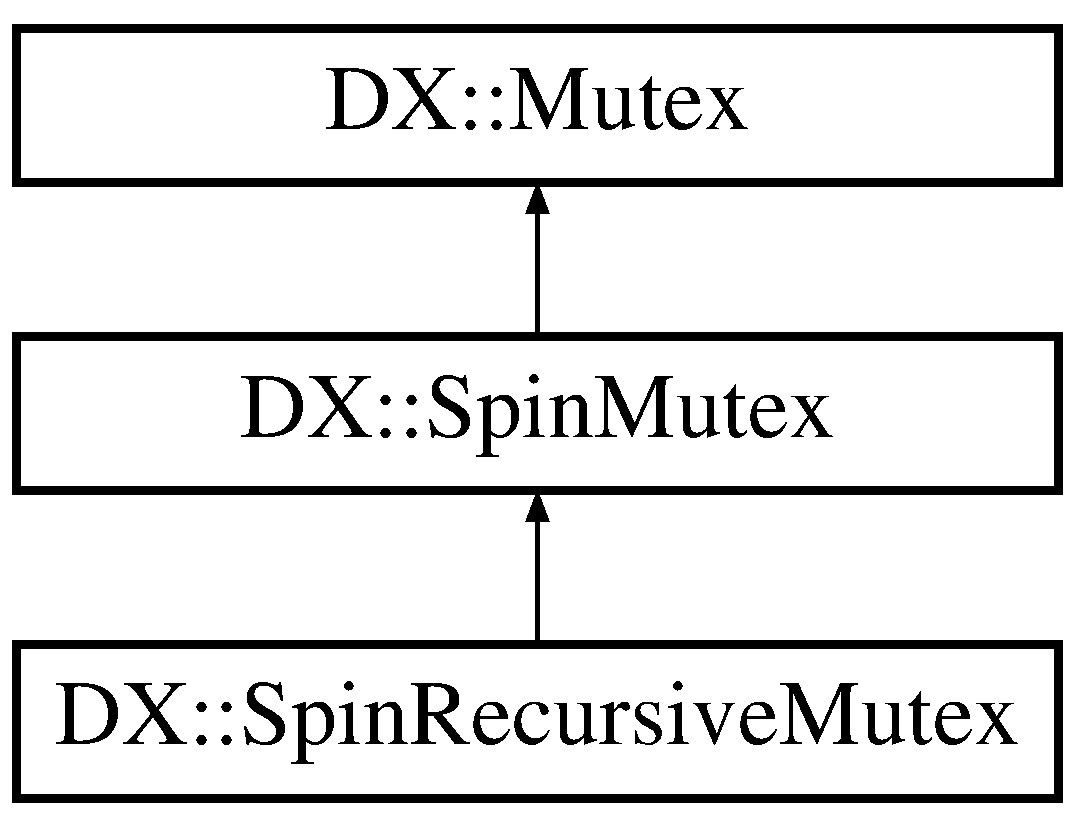
\includegraphics[height=3.000000cm]{class_d_x_1_1_spin_recursive_mutex}
\end{center}
\end{figure}
\subsection*{Public Member Functions}
\begin{DoxyCompactItemize}
\item 
void \hyperlink{class_d_x_1_1_spin_recursive_mutex_a928053922f1a59db49d6027d108b88ba}{lock} () const 
\begin{DoxyCompactList}\small\item\em Locks the mutex. Further calls to lock will block until there is a call to \hyperlink{class_d_x_1_1_spin_recursive_mutex_aa470bb06feb399e8771296a79b888287}{unlock()}. \end{DoxyCompactList}\item 
bool \hyperlink{class_d_x_1_1_spin_recursive_mutex_a9150334e2741a1de69f177491214cf15}{try\-Lock} () const 
\begin{DoxyCompactList}\small\item\em Attempts to lock the mutex. \hyperlink{class_d_x_1_1_spin_recursive_mutex_a9150334e2741a1de69f177491214cf15}{try\-Lock()} is non-\/blocking, meaning that regardless of the state of the mutex when \hyperlink{class_d_x_1_1_spin_recursive_mutex_a9150334e2741a1de69f177491214cf15}{try\-Lock()} is called, execution will continue. \end{DoxyCompactList}\item 
\hypertarget{class_d_x_1_1_spin_recursive_mutex_aa470bb06feb399e8771296a79b888287}{void \hyperlink{class_d_x_1_1_spin_recursive_mutex_aa470bb06feb399e8771296a79b888287}{unlock} () const }\label{class_d_x_1_1_spin_recursive_mutex_aa470bb06feb399e8771296a79b888287}

\begin{DoxyCompactList}\small\item\em Unlocks the mutex. This call is non-\/blocking, because having it otherwise doesn't make any sense. \end{DoxyCompactList}\end{DoxyCompactItemize}
\subsection*{Additional Inherited Members}


\subsection{Member Function Documentation}
\hypertarget{class_d_x_1_1_spin_recursive_mutex_a928053922f1a59db49d6027d108b88ba}{\index{D\-X\-::\-Spin\-Recursive\-Mutex@{D\-X\-::\-Spin\-Recursive\-Mutex}!lock@{lock}}
\index{lock@{lock}!DX::SpinRecursiveMutex@{D\-X\-::\-Spin\-Recursive\-Mutex}}
\subsubsection[{lock}]{\setlength{\rightskip}{0pt plus 5cm}void D\-X\-::\-Spin\-Recursive\-Mutex\-::lock (
\begin{DoxyParamCaption}
{}
\end{DoxyParamCaption}
) const\hspace{0.3cm}{\ttfamily [virtual]}}}\label{class_d_x_1_1_spin_recursive_mutex_a928053922f1a59db49d6027d108b88ba}


Locks the mutex. Further calls to lock will block until there is a call to \hyperlink{class_d_x_1_1_spin_recursive_mutex_aa470bb06feb399e8771296a79b888287}{unlock()}. 

\begin{DoxyNote}{Note}
\hyperlink{class_d_x_1_1_spin_recursive_mutex_a928053922f1a59db49d6027d108b88ba}{lock()} is not recursive. 

\hyperlink{class_d_x_1_1_spin_recursive_mutex_a928053922f1a59db49d6027d108b88ba}{lock()} is blocking. 
\end{DoxyNote}


Reimplemented from \hyperlink{class_d_x_1_1_spin_mutex_a2237431b7beabcff6936a375c3b41f00}{D\-X\-::\-Spin\-Mutex}.

\hypertarget{class_d_x_1_1_spin_recursive_mutex_a9150334e2741a1de69f177491214cf15}{\index{D\-X\-::\-Spin\-Recursive\-Mutex@{D\-X\-::\-Spin\-Recursive\-Mutex}!try\-Lock@{try\-Lock}}
\index{try\-Lock@{try\-Lock}!DX::SpinRecursiveMutex@{D\-X\-::\-Spin\-Recursive\-Mutex}}
\subsubsection[{try\-Lock}]{\setlength{\rightskip}{0pt plus 5cm}bool D\-X\-::\-Spin\-Recursive\-Mutex\-::try\-Lock (
\begin{DoxyParamCaption}
{}
\end{DoxyParamCaption}
) const\hspace{0.3cm}{\ttfamily [virtual]}}}\label{class_d_x_1_1_spin_recursive_mutex_a9150334e2741a1de69f177491214cf15}


Attempts to lock the mutex. \hyperlink{class_d_x_1_1_spin_recursive_mutex_a9150334e2741a1de69f177491214cf15}{try\-Lock()} is non-\/blocking, meaning that regardless of the state of the mutex when \hyperlink{class_d_x_1_1_spin_recursive_mutex_a9150334e2741a1de69f177491214cf15}{try\-Lock()} is called, execution will continue. 

\begin{DoxyNote}{Note}
\hyperlink{class_d_x_1_1_spin_recursive_mutex_a9150334e2741a1de69f177491214cf15}{try\-Lock()} is not recursive. 

\hyperlink{class_d_x_1_1_spin_recursive_mutex_a9150334e2741a1de69f177491214cf15}{try\-Lock()} is non-\/blocking. 
\end{DoxyNote}


Reimplemented from \hyperlink{class_d_x_1_1_spin_mutex_af1a59657616a8c68ff5785e18e53a469}{D\-X\-::\-Spin\-Mutex}.



The documentation for this class was generated from the following files\-:\begin{DoxyCompactItemize}
\item 
Mutex/Spin\-Recursive\-Mutex.\-h\item 
Mutex/Spin\-Recursive\-Mutex.\-cpp\end{DoxyCompactItemize}

\hypertarget{class_d_x_1_1_spin_r_w_lock}{\section{D\-X\-:\-:Spin\-R\-W\-Lock Class Reference}
\label{class_d_x_1_1_spin_r_w_lock}\index{D\-X\-::\-Spin\-R\-W\-Lock@{D\-X\-::\-Spin\-R\-W\-Lock}}
}


\hyperlink{class_d_x_1_1_spin_r_w_lock}{Spin\-R\-W\-Lock} is the preferred way of interacting with a \hyperlink{class_d_x_1_1_spin_r_w_mutex}{Spin\-R\-W\-Mutex}. \hyperlink{class_d_x_1_1_spin_r_w_lock}{Spin\-R\-W\-Lock} is a lock-\/guard style class, locking the \hyperlink{class_d_x_1_1_spin_r_w_mutex}{Spin\-R\-W\-Mutex} upon construction and releasing the lock upon destruction. \hyperlink{class_d_x_1_1_spin_r_w_mutex}{Spin\-R\-W\-Mutex} remembers whether it is a reader or writer lock, and releases the same kind of lock that it was constructed with.  




{\ttfamily \#include $<$Spin\-R\-W\-Mutex.\-h$>$}

\subsection*{Public Member Functions}
\begin{DoxyCompactItemize}
\item 
\hyperlink{class_d_x_1_1_spin_r_w_lock_a031480610e0da0bd664ada662057b99c}{Spin\-R\-W\-Lock} (const \hyperlink{class_d_x_1_1_spin_r_w_mutex}{Spin\-R\-W\-Mutex} \&mutex, bool is\-Writer)
\end{DoxyCompactItemize}


\subsection{Detailed Description}
\hyperlink{class_d_x_1_1_spin_r_w_lock}{Spin\-R\-W\-Lock} is the preferred way of interacting with a \hyperlink{class_d_x_1_1_spin_r_w_mutex}{Spin\-R\-W\-Mutex}. \hyperlink{class_d_x_1_1_spin_r_w_lock}{Spin\-R\-W\-Lock} is a lock-\/guard style class, locking the \hyperlink{class_d_x_1_1_spin_r_w_mutex}{Spin\-R\-W\-Mutex} upon construction and releasing the lock upon destruction. \hyperlink{class_d_x_1_1_spin_r_w_mutex}{Spin\-R\-W\-Mutex} remembers whether it is a reader or writer lock, and releases the same kind of lock that it was constructed with. 

The big advantage of using Spin\-R\-W\-Locks over \hyperlink{class_d_x_1_1_spin_r_w_mutex}{Spin\-R\-W\-Mutex} is the automatic unlock on destruction\-: unlike the examples provided above, no copies have to be made on a get() call

\begin{DoxyNote}{Note}
Spin\-R\-W\-Locks do not allow for recursive writer-\/locks of a single \hyperlink{class_d_x_1_1_spin_r_w_mutex}{Spin\-R\-W\-Mutex}
\end{DoxyNote}

\begin{DoxyCode}
MyClass myClass;
\textcolor{keyword}{mutable} SpinRWMutex myRWMutex;

MyClass getMyClass()\textcolor{keyword}{ const}
\textcolor{keyword}{}\{
    \hyperlink{class_d_x_1_1_spin_r_w_lock_a031480610e0da0bd664ada662057b99c}{SpinRWLock} \_lock(myRWMutex, \textcolor{keyword}{false});
    \textcolor{keywordflow}{return} myClass; \textcolor{comment}{// No copies or thread-local storage necessary}
\}

\textcolor{keywordtype}{void} setMyClass(\textcolor{keyword}{const} MyClass& other)
\{
    \hyperlink{class_d_x_1_1_spin_r_w_lock_a031480610e0da0bd664ada662057b99c}{SpinRWLock} \_lock(myRWMutex, \textcolor{keyword}{true});
    myClass = other;
\}
\end{DoxyCode}
 

\subsection{Constructor \& Destructor Documentation}
\hypertarget{class_d_x_1_1_spin_r_w_lock_a031480610e0da0bd664ada662057b99c}{\index{D\-X\-::\-Spin\-R\-W\-Lock@{D\-X\-::\-Spin\-R\-W\-Lock}!Spin\-R\-W\-Lock@{Spin\-R\-W\-Lock}}
\index{Spin\-R\-W\-Lock@{Spin\-R\-W\-Lock}!DX::SpinRWLock@{D\-X\-::\-Spin\-R\-W\-Lock}}
\subsubsection[{Spin\-R\-W\-Lock}]{\setlength{\rightskip}{0pt plus 5cm}D\-X\-::\-Spin\-R\-W\-Lock\-::\-Spin\-R\-W\-Lock (
\begin{DoxyParamCaption}
\item[{const {\bf Spin\-R\-W\-Mutex} \&}]{mutex, }
\item[{bool}]{is\-Writer}
\end{DoxyParamCaption}
)}}\label{class_d_x_1_1_spin_r_w_lock_a031480610e0da0bd664ada662057b99c}

\begin{DoxyParams}[1]{Parameters}
\mbox{\tt in}  & {\em mutex} & The \hyperlink{class_d_x_1_1_spin_r_w_mutex}{Spin\-R\-W\-Mutex} that the lock should be locking/unlocking \\
\hline
\mbox{\tt in}  & {\em is\-Writer} & True indicates a writer lock, False indicates a reader lock \\
\hline
\end{DoxyParams}


The documentation for this class was generated from the following files\-:\begin{DoxyCompactItemize}
\item 
Mutex/Spin\-R\-W\-Mutex.\-h\item 
Mutex/Spin\-R\-W\-Mutex.\-cpp\end{DoxyCompactItemize}

\hypertarget{class_d_x_1_1_spin_r_w_mutex}{\section{D\-X\-:\-:Spin\-R\-W\-Mutex Class Reference}
\label{class_d_x_1_1_spin_r_w_mutex}\index{D\-X\-::\-Spin\-R\-W\-Mutex@{D\-X\-::\-Spin\-R\-W\-Mutex}}
}


\hyperlink{class_d_x_1_1_spin_r_w_mutex}{Spin\-R\-W\-Mutex} is a leightweight mutex that supports multiple readers (const-\/only access) and a single writer. Supports readers up to the maximum value of size\-\_\-t for your system.  




{\ttfamily \#include $<$Spin\-Locks.\-h$>$}

\subsection*{Public Member Functions}
\begin{DoxyCompactItemize}
\item 
void \hyperlink{class_d_x_1_1_spin_r_w_mutex_ac2b4ebd8c8bd297c5e2d907c92c75a56}{lock} (bool is\-Writer)
\begin{DoxyCompactList}\small\item\em Locks the mutex as a writer or a reader. \end{DoxyCompactList}\item 
\hypertarget{class_d_x_1_1_spin_r_w_mutex_ac82ed966423779e8e021cf8a227ca4d9}{void \hyperlink{class_d_x_1_1_spin_r_w_mutex_ac82ed966423779e8e021cf8a227ca4d9}{unlock} (bool is\-Writer)}\label{class_d_x_1_1_spin_r_w_mutex_ac82ed966423779e8e021cf8a227ca4d9}

\begin{DoxyCompactList}\small\item\em Unlocks the mutex as a writer or a reader. \end{DoxyCompactList}\end{DoxyCompactItemize}


\subsection{Detailed Description}
\hyperlink{class_d_x_1_1_spin_r_w_mutex}{Spin\-R\-W\-Mutex} is a leightweight mutex that supports multiple readers (const-\/only access) and a single writer. Supports readers up to the maximum value of size\-\_\-t for your system. 

Calls to \hyperlink{class_d_x_1_1_spin_r_w_mutex_ac2b4ebd8c8bd297c5e2d907c92c75a56}{lock()} from readers will block if a writer holds the lock. Calls to \hyperlink{class_d_x_1_1_spin_r_w_mutex_ac2b4ebd8c8bd297c5e2d907c92c75a56}{lock()} from writers will block if there are any readers or writers holding onto the lock.

\begin{DoxyNote}{Note}
\hyperlink{class_d_x_1_1_spin_r_w_mutex}{Spin\-R\-W\-Mutex} is favored towards writers attempting to get the lock

\hyperlink{class_d_x_1_1_spin_r_w_mutex}{Spin\-R\-W\-Mutex} is easiest to use with \hyperlink{class_d_x_1_1_spin_r_w_lock}{Spin\-R\-W\-Lock}. \hyperlink{class_d_x_1_1_spin_r_w_lock}{Spin\-R\-W\-Lock} lets you \char`\"{}set-\/it-\/and-\/forget-\/it\char`\"{} in regards to remembering if you're a reader/writer.

\hyperlink{class_d_x_1_1_spin_r_w_mutex}{Spin\-R\-W\-Mutex} does {\itshape N\-O\-T} check to ensure that calls to lock/unlock are called with the same boolean. It does handle these cases (crash-\/wise), but calling lock(true) and unlock(false) from the same thread does not unlock the writer lock.
\end{DoxyNote}

\begin{DoxyCode}
\textcolor{keyword}{mutable} SpinRWMutex myRWMutex;
MyClass myClass;

\textcolor{keywordtype}{void} setMyClass(\textcolor{keyword}{const} MyClass& other)
\{
    myRWMutex.lock(\textcolor{keyword}{true}); \textcolor{comment}{// true indicates a writer}
    myClass = other;
    myRWMutex.unlock(\textcolor{keyword}{true}); \textcolor{comment}{// unlock my writer reference            }
\}

MyClass getMyClass()\textcolor{keyword}{ const}
\textcolor{keyword}{}\{
    \textcolor{comment}{// static , thread-local object so it isn't constructed every function call, only copied}
    \textcolor{keyword}{static} thread\_local MyClass ret;
    myRWMutex.lock(\textcolor{keyword}{false}); \textcolor{comment}{// false indicates reader}
    ret = myClass;
    myRwMutex.unlock(\textcolor{keyword}{false}); \textcolor{comment}{// unlock my reader reference}
    \textcolor{keywordflow}{return} ret;
\}
\end{DoxyCode}
 

\subsection{Member Function Documentation}
\hypertarget{class_d_x_1_1_spin_r_w_mutex_ac2b4ebd8c8bd297c5e2d907c92c75a56}{\index{D\-X\-::\-Spin\-R\-W\-Mutex@{D\-X\-::\-Spin\-R\-W\-Mutex}!lock@{lock}}
\index{lock@{lock}!DX::SpinRWMutex@{D\-X\-::\-Spin\-R\-W\-Mutex}}
\subsubsection[{lock}]{\setlength{\rightskip}{0pt plus 5cm}void D\-X\-::\-Spin\-R\-W\-Mutex\-::lock (
\begin{DoxyParamCaption}
\item[{bool}]{is\-Writer}
\end{DoxyParamCaption}
)}}\label{class_d_x_1_1_spin_r_w_mutex_ac2b4ebd8c8bd297c5e2d907c92c75a56}


Locks the mutex as a writer or a reader. 


\begin{DoxyParams}[1]{Parameters}
\mbox{\tt in}  & {\em is\-Writer} & true indicates the caller is attempting to lock this as a writer, false indicates the caller is attempting to lock as a reader. \\
\hline
\end{DoxyParams}
\begin{DoxyNote}{Note}
\hyperlink{class_d_x_1_1_spin_r_w_mutex_ac2b4ebd8c8bd297c5e2d907c92c75a56}{lock()} is not recursive. 

\hyperlink{class_d_x_1_1_spin_r_w_mutex_ac2b4ebd8c8bd297c5e2d907c92c75a56}{lock()} is blocking. 
\end{DoxyNote}


The documentation for this class was generated from the following file\-:\begin{DoxyCompactItemize}
\item 
Mutex/Spin\-Locks.\-h\end{DoxyCompactItemize}

\hypertarget{class_d_x_1_1_spin_yield_mutex}{\section{D\-X\-:\-:Spin\-Yield\-Mutex Class Reference}
\label{class_d_x_1_1_spin_yield_mutex}\index{D\-X\-::\-Spin\-Yield\-Mutex@{D\-X\-::\-Spin\-Yield\-Mutex}}
}
Inheritance diagram for D\-X\-:\-:Spin\-Yield\-Mutex\-:\begin{figure}[H]
\begin{center}
\leavevmode
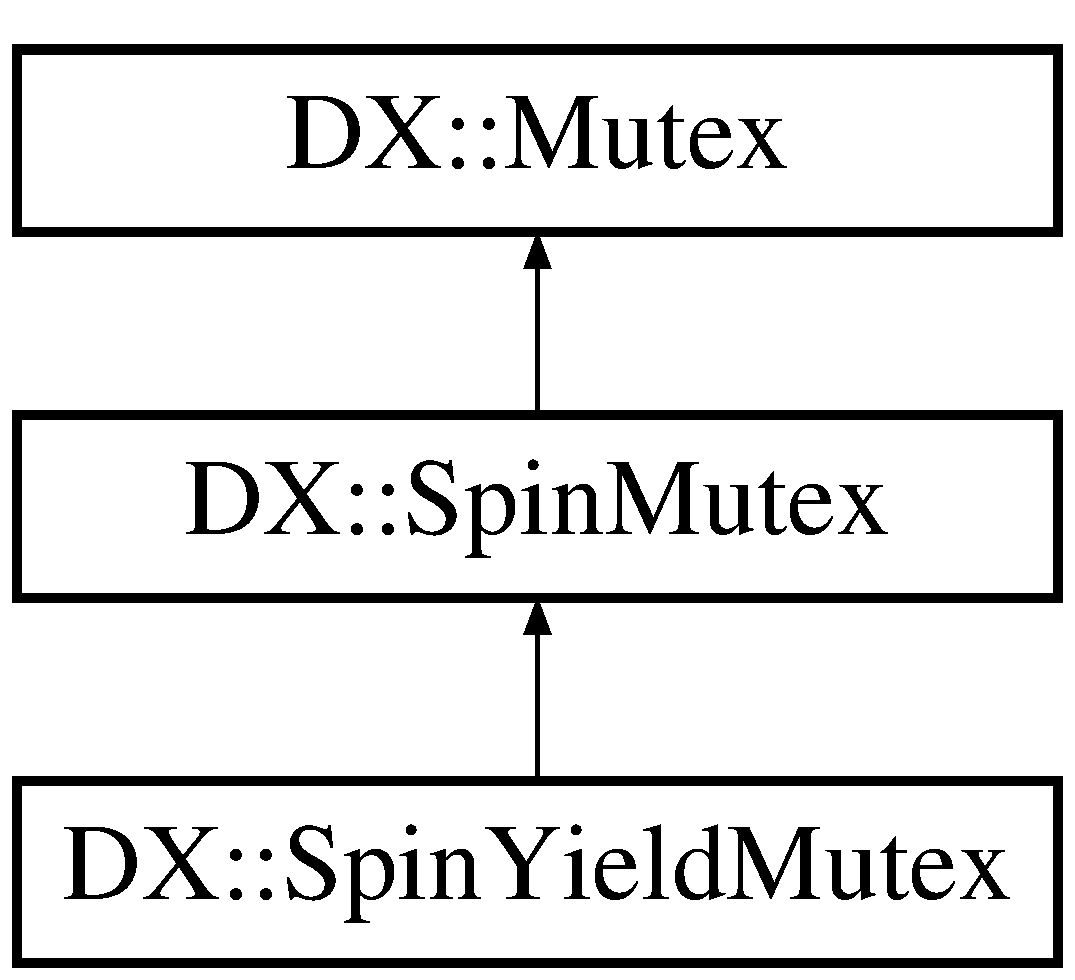
\includegraphics[height=3.000000cm]{class_d_x_1_1_spin_yield_mutex}
\end{center}
\end{figure}
\subsection*{Public Member Functions}
\begin{DoxyCompactItemize}
\item 
\hypertarget{class_d_x_1_1_spin_yield_mutex_a039edcf6c2266ace07dfa648f9a45f78}{{\bfseries Spin\-Yield\-Mutex} (const size\-\_\-t max\-Yield\-Ticks=D\-E\-F\-A\-U\-L\-T\-\_\-\-Y\-I\-E\-L\-D\-\_\-\-T\-I\-C\-K\-S)}\label{class_d_x_1_1_spin_yield_mutex_a039edcf6c2266ace07dfa648f9a45f78}

\item 
void \hyperlink{class_d_x_1_1_spin_yield_mutex_ad2229f4e9acd7c6bab9e2fbe029b1f1f}{lock} () const 
\begin{DoxyCompactList}\small\item\em Locks the mutex. Further calls to lock will block until there is a call to \hyperlink{class_d_x_1_1_spin_yield_mutex_a89bd23cc61dc3029baf5b2c14f834dfc}{unlock()}. \end{DoxyCompactList}\item 
bool \hyperlink{class_d_x_1_1_spin_yield_mutex_acd1ed560cf8afd7363a520beff4b5455}{try\-Lock} () const 
\begin{DoxyCompactList}\small\item\em Attempts to lock the mutex. \hyperlink{class_d_x_1_1_spin_yield_mutex_acd1ed560cf8afd7363a520beff4b5455}{try\-Lock()} is non-\/blocking, meaning that regardless of the state of the mutex when \hyperlink{class_d_x_1_1_spin_yield_mutex_acd1ed560cf8afd7363a520beff4b5455}{try\-Lock()} is called, execution will continue. \end{DoxyCompactList}\item 
\hypertarget{class_d_x_1_1_spin_yield_mutex_a89bd23cc61dc3029baf5b2c14f834dfc}{void \hyperlink{class_d_x_1_1_spin_yield_mutex_a89bd23cc61dc3029baf5b2c14f834dfc}{unlock} () const }\label{class_d_x_1_1_spin_yield_mutex_a89bd23cc61dc3029baf5b2c14f834dfc}

\begin{DoxyCompactList}\small\item\em Unlocks the mutex. This call is non-\/blocking, because having it otherwise doesn't make any sense. \end{DoxyCompactList}\end{DoxyCompactItemize}
\subsection*{Additional Inherited Members}


\subsection{Member Function Documentation}
\hypertarget{class_d_x_1_1_spin_yield_mutex_ad2229f4e9acd7c6bab9e2fbe029b1f1f}{\index{D\-X\-::\-Spin\-Yield\-Mutex@{D\-X\-::\-Spin\-Yield\-Mutex}!lock@{lock}}
\index{lock@{lock}!DX::SpinYieldMutex@{D\-X\-::\-Spin\-Yield\-Mutex}}
\subsubsection[{lock}]{\setlength{\rightskip}{0pt plus 5cm}void D\-X\-::\-Spin\-Yield\-Mutex\-::lock (
\begin{DoxyParamCaption}
{}
\end{DoxyParamCaption}
) const\hspace{0.3cm}{\ttfamily [virtual]}}}\label{class_d_x_1_1_spin_yield_mutex_ad2229f4e9acd7c6bab9e2fbe029b1f1f}


Locks the mutex. Further calls to lock will block until there is a call to \hyperlink{class_d_x_1_1_spin_yield_mutex_a89bd23cc61dc3029baf5b2c14f834dfc}{unlock()}. 

\begin{DoxyNote}{Note}
\hyperlink{class_d_x_1_1_spin_yield_mutex_ad2229f4e9acd7c6bab9e2fbe029b1f1f}{lock()} is not recursive. 

\hyperlink{class_d_x_1_1_spin_yield_mutex_ad2229f4e9acd7c6bab9e2fbe029b1f1f}{lock()} is blocking. 
\end{DoxyNote}


Reimplemented from \hyperlink{class_d_x_1_1_spin_mutex_a133720662c9262696659d4dcd6d3adec}{D\-X\-::\-Spin\-Mutex}.

\hypertarget{class_d_x_1_1_spin_yield_mutex_acd1ed560cf8afd7363a520beff4b5455}{\index{D\-X\-::\-Spin\-Yield\-Mutex@{D\-X\-::\-Spin\-Yield\-Mutex}!try\-Lock@{try\-Lock}}
\index{try\-Lock@{try\-Lock}!DX::SpinYieldMutex@{D\-X\-::\-Spin\-Yield\-Mutex}}
\subsubsection[{try\-Lock}]{\setlength{\rightskip}{0pt plus 5cm}bool D\-X\-::\-Spin\-Yield\-Mutex\-::try\-Lock (
\begin{DoxyParamCaption}
{}
\end{DoxyParamCaption}
) const\hspace{0.3cm}{\ttfamily [virtual]}}}\label{class_d_x_1_1_spin_yield_mutex_acd1ed560cf8afd7363a520beff4b5455}


Attempts to lock the mutex. \hyperlink{class_d_x_1_1_spin_yield_mutex_acd1ed560cf8afd7363a520beff4b5455}{try\-Lock()} is non-\/blocking, meaning that regardless of the state of the mutex when \hyperlink{class_d_x_1_1_spin_yield_mutex_acd1ed560cf8afd7363a520beff4b5455}{try\-Lock()} is called, execution will continue. 

\begin{DoxyNote}{Note}
\hyperlink{class_d_x_1_1_spin_yield_mutex_acd1ed560cf8afd7363a520beff4b5455}{try\-Lock()} is not recursive. 

\hyperlink{class_d_x_1_1_spin_yield_mutex_acd1ed560cf8afd7363a520beff4b5455}{try\-Lock()} is non-\/blocking. 
\end{DoxyNote}


Reimplemented from \hyperlink{class_d_x_1_1_spin_mutex_a395c28ec936bce90ac562039168a540a}{D\-X\-::\-Spin\-Mutex}.



The documentation for this class was generated from the following file\-:\begin{DoxyCompactItemize}
\item 
Mutex/Spin\-Locks.\-h\end{DoxyCompactItemize}

\hypertarget{class_d_x_1_1_std_lock}{\section{D\-X\-:\-:Std\-Lock Class Reference}
\label{class_d_x_1_1_std_lock}\index{D\-X\-::\-Std\-Lock@{D\-X\-::\-Std\-Lock}}
}
\subsection*{Public Member Functions}
\begin{DoxyCompactItemize}
\item 
\hypertarget{class_d_x_1_1_std_lock_a0c37e2db9c2f36346c615e78509ad206}{{\bfseries Std\-Lock} (std\-::mutex \&\-\_\-mutex)}\label{class_d_x_1_1_std_lock_a0c37e2db9c2f36346c615e78509ad206}

\end{DoxyCompactItemize}


The documentation for this class was generated from the following file\-:\begin{DoxyCompactItemize}
\item 
Mutex/Std\-Locks.\-h\end{DoxyCompactItemize}

%--- End generated contents ---

% Index
\newpage
\phantomsection
\addcontentsline{toc}{chapter}{Index}
\printindex

\end{document}
